\documentclass[tikz]{standalone}
\usepackage[outline]{contour}

\begin{document}
	    \contourlength{1.5pt}
	    
	    \tikzset{
	    	double arrow/.style args={#1 colored by #2 and #3}{
	    		-stealth,line width=#1,#2, % first arrow
	    		postaction={draw,-stealth,#3,line width=(#1)/3,
	    			shorten <=(#1)/3,shorten >=2*(#1)/3}, % second arrow
	    	}
	    }
\begin{tikzpicture}
    \node[anchor=south west,inner sep=0] at (0,0) {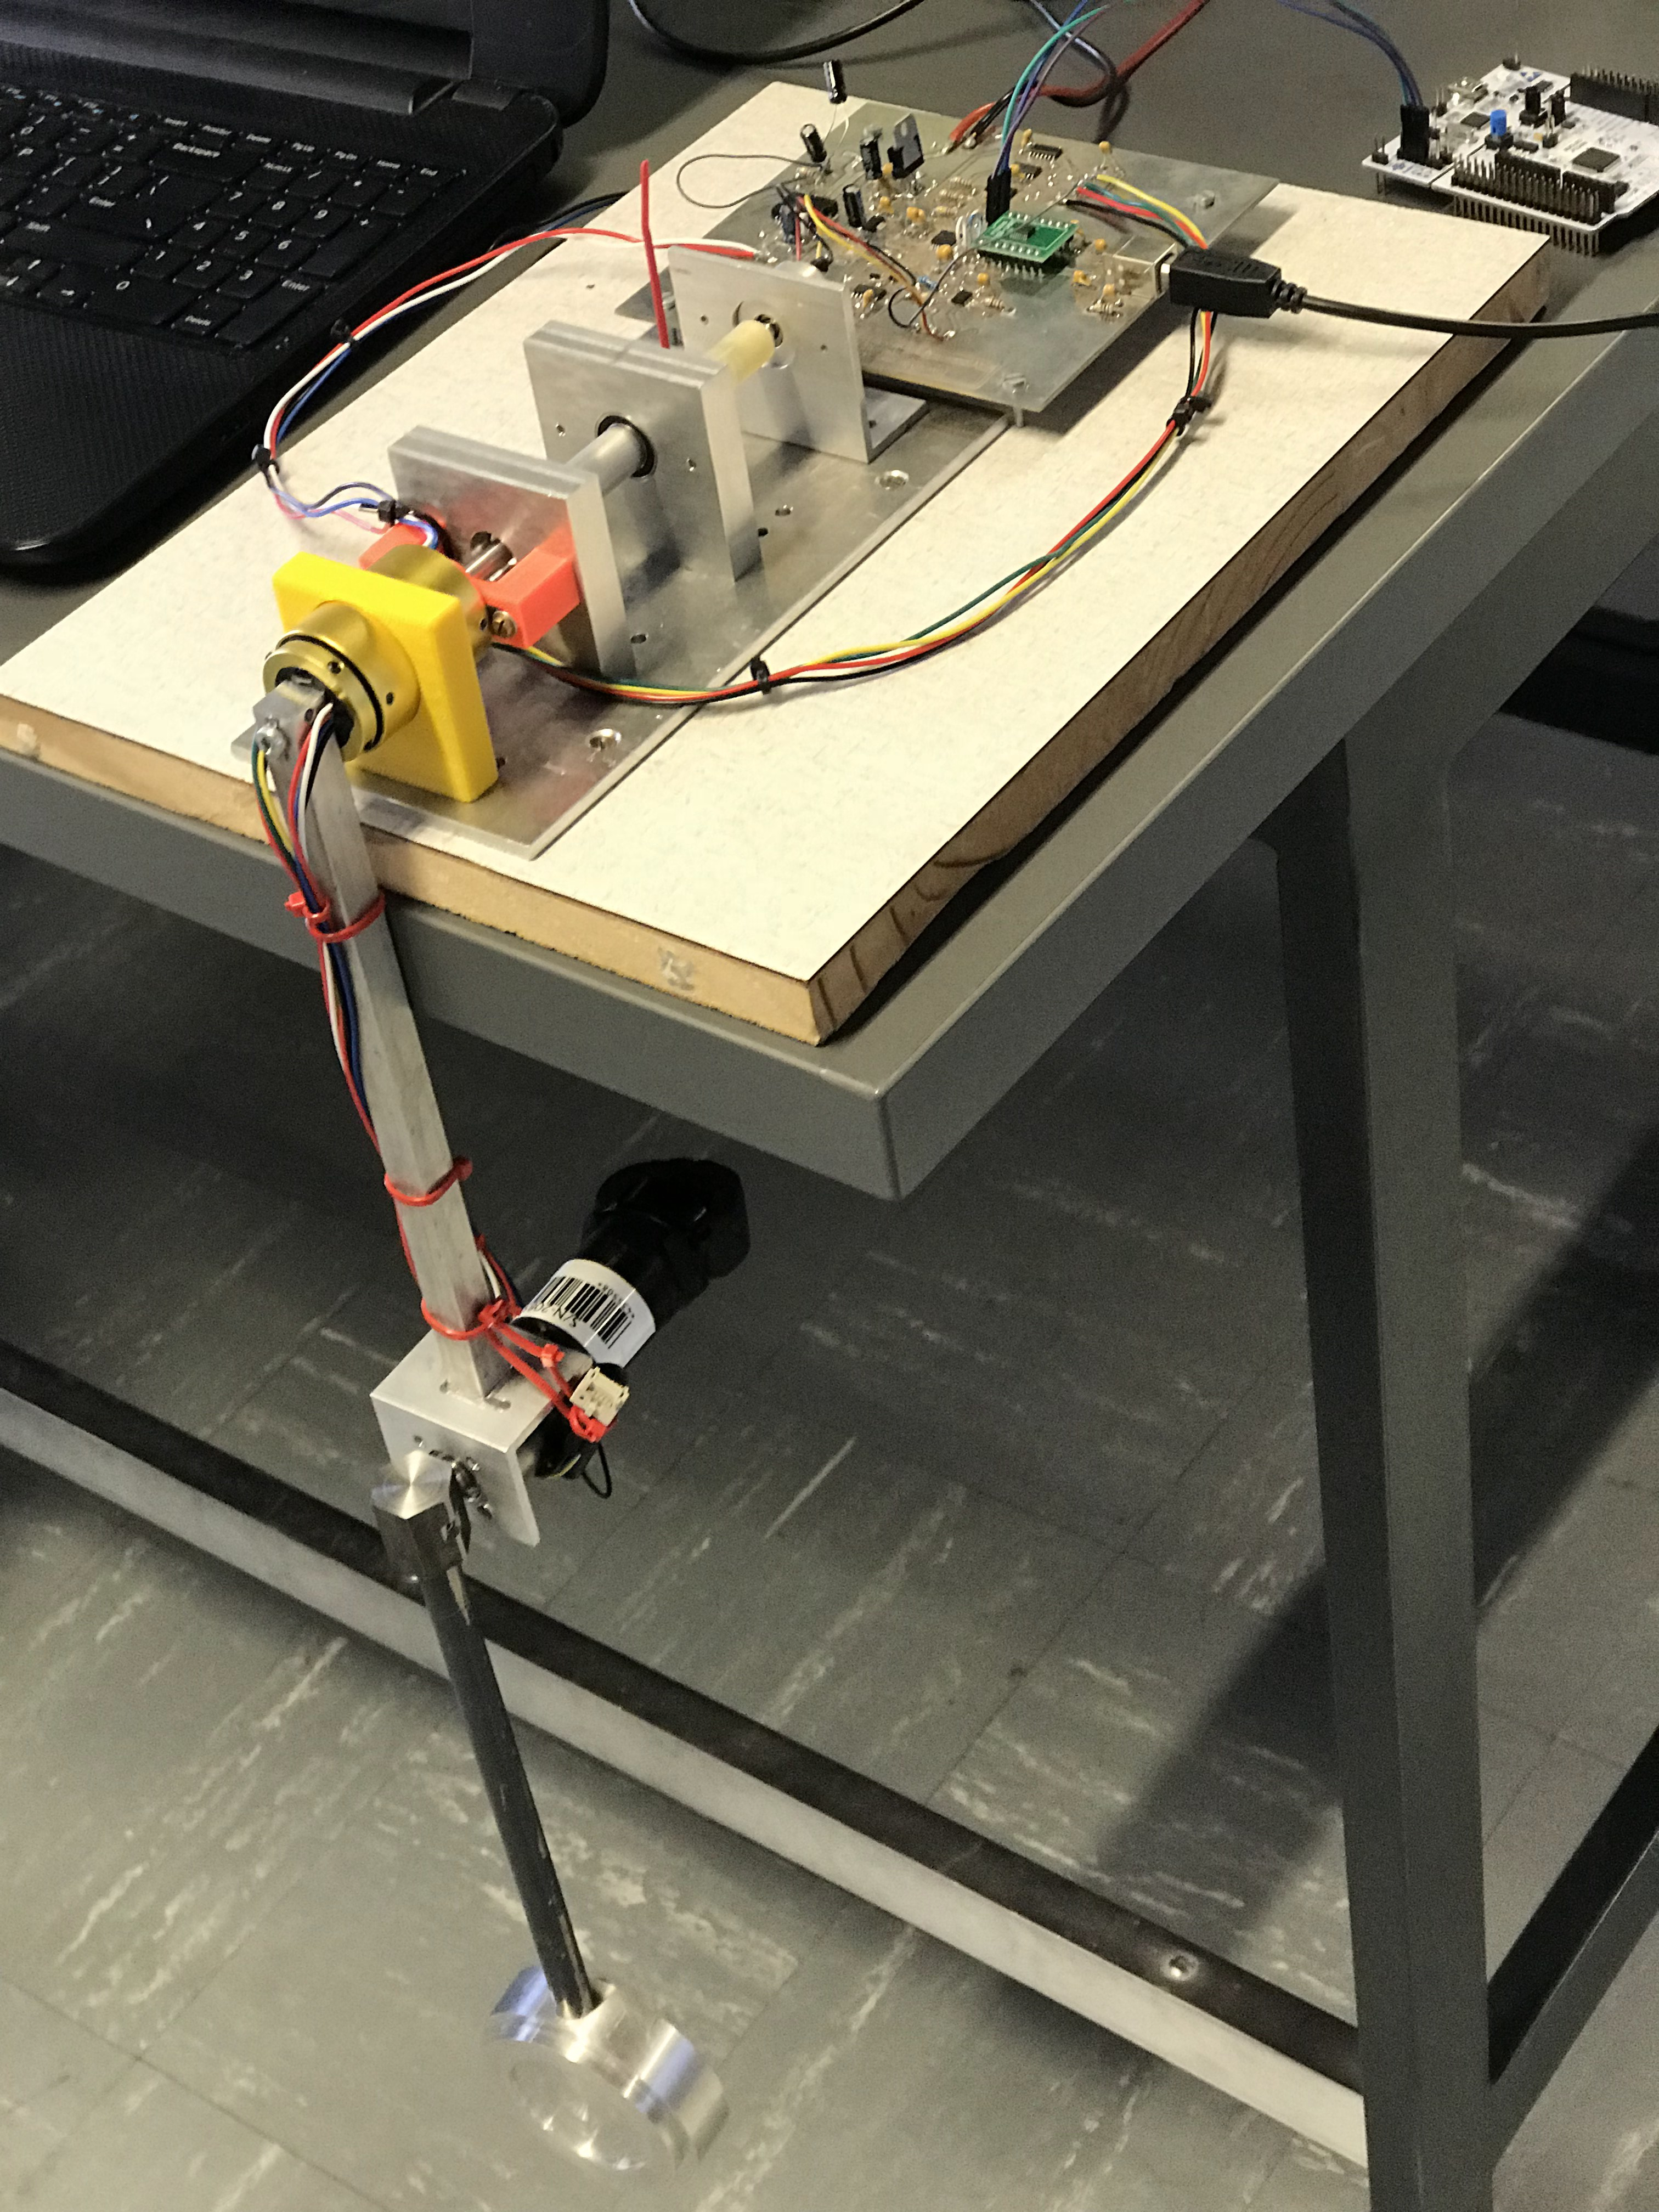
\includegraphics[width=\textwidth]{mech.jpg}};
    %microcontroller
    %\draw[green,ultra thick,rounded corners] (6.5,5) node[above]{ \textbf{MCU} };
    
	\draw[double arrow=2pt colored by black and white] (8,2) node[right,black]{\contour{white}{\textbf{Point Mass}} } -- (4.5,0.8) ;
	
	\draw[double arrow=2pt colored by black and white] (8,3) node[right,black]{\contour{white}{\textbf{Actuated Pendulum}}} --(3.8,3) ;
	
	\draw[double arrow=2pt colored by black and white] (8,4) node[right,black]{\contour{white}{\textbf{Motor Mounting}}} -- (3.8,6) ;
	
	\draw[double arrow=2pt colored by black and white] (8,5)node[right,black]{\contour{white}{\textbf{DC Motor}}} --(4.5,6.5)  ;
	
	\draw[double arrow=2pt colored by black and white] (8,6)node[right,black]{\contour{white}{\textbf{Encoder}}} -- (5,7) ;
    
    \draw[double arrow=2pt colored by black and white] (8,7)node[right,black]{\contour{white}{\textbf{Unactuated Pendulum}}} -- (2.8,9) ;
    
    \draw[double arrow=2pt colored by black and white] (8,8)node[right,black]{\contour{white}{\textbf{Slipring}}} -- (2.8,11)  ;
    
    \draw[double arrow=2pt colored by black and white] (8,9)node[right,black]{\contour{white}{\textbf{Bearing Housing}}} -- (3.5,12.5) ;
    
    \draw[double arrow=2pt colored by black and white] (8,10) node[right,black]{\contour{white}{\textbf{Shaft}}} -- (4.4,12.8) ;
    
    \draw[double arrow=2pt colored by black and white] (8,11)node[right,black]{\contour{white}{\textbf{Rubber Coupling}}} -- (5.5,13.5);
    
    \draw[double arrow=2pt colored by black and white] (8,12)node[right,black]{\contour{white}{\textbf{Potentiometer}}} --  (5.8,14.2);
    
    
\end{tikzpicture}
\end{document}